\section{Introduction}

This exposition gives an overview of the Elmer software package. General information 
on the capabilities of the software, its usage, and how the material of the package 
is organized is presented. More detailed information is given
in the other Elmer manuals, the scopes of which are described in this document.
%The emphasis is on the total view
%and the user is encouraged to read the other Elmer manuals for more detailed information. 

\subsection*{What is Elmer}

Elmer is a finite element software package for the solution of partial differential 
equations. Elmer can deal with a great number of different equations, which may be coupled 
in a generic manner making Elmer a versatile tool for multiphysical simulations. 
As an open source software, Elmer also gives the user the means to modify the existing 
solution procedures and to develop new solvers for equations of interest to the user.  

\subsection*{History of Elmer}
The development of Elmer was started in 1995 as part of a national CFD technology 
program funded by the Finnish funding agency for technology and innovation, Tekes. 
The original development consortia included partners from CSC - The Finnish IT Center 
for Science, Helsinki University of Technology TKK, VTT Technical Research Centre of Finland,
University of Jyv�skyl�, and Okmetic Ltd. After the five years initial project ended 
the development has been continued by CSC in different application fields.

\subsection*{Licensing}
In September 2005 Elmer was released under GNU General Public License (GPL). This 
has widened the user community, particularly the number of international users has grown.
%meant a significant growth particularly of the international user community. 
However, as the sole owner of the copyright to Elmer source code, CSC may distribute 
Elmer also under other licensing terms. Therefore, if GPL does not suit your purposes, 
you may contact the Elmer team for other licensing options. 

\subsection*{Distribution}
Elmer is distributed only through the Internet. The actual distribution site may vary 
but the pointer to the location may always be found at \URL{http://www.csc.fi/elmer}. 

The distribution of Elmer comes in three different parts: sources, binaries, and documentation.
Unix users are encouraged to 
compile the software themselves. The compilation instructions are given at the www-page.
For Windows and Macintosh a precompiled binary version of the code is also provided. 
The documentation of the software is already quite extensive, but unfortunately still not complete.


\section{Key features of Elmer}

Elmer offers a wide range of methods and techniques for the computational modeling of
physical phenomena described by partial differential equations.
In the following some of the most essential ones are summarized.
%Elmer includes a huge number of capabilities in different categories. This list summarizes 
%some of the most essential ones.

\subsection*{Physical models in Elmer}
The Elmer package contains solvers for a variety of mathematical models.
The following list summarizes the capabilities of Elmer in specialized fields.
\begin{itemize}
  \item Heat transfer: models for conduction, radiation and phase change
  \item Fluid flow: the Navier-Stokes, Stokes and Reynolds equations, k-$\varepsilon$ model
  \item Species transport: generic convection-diffusion equation
  \item Elasticity: general elasticity equations, dimensionally reduced models for plates and shells
  \item Acoustics: the Helmholtz equation
  \item Electromagnetism: electrostatics, magnetostatics, induction
  \item Microfluidics: slip conditions, the Poisson-Boltzmann equation
  \item Levelset method: Eulerian free boundary problems 
  \item Quantum Mechanics: density functional theory (Kohn-Sham)
\end{itemize}

\subsection*{Numerical methods in Elmer}

For approximation and linear system solution Elmer offers a great number of possibilities.
The following list summarizes some of the most essential ones.

\begin{itemize}
  \item All basic element shapes in 1D, 2D and 3D with the Lagrange shape functions
of degree $k \le 2$
%All basic Langrangian elementtypes in 1D, 2D and 3D in 1st and 2nd degree
  \item Higher degree approximation using $p$-elements
%Generic p-base elements
  \item Time integration schemes for the first and second order equations
  \item Solution methods for eigenvalue problems
  \item Direct linear system solvers (Lapack \& Umfpack)
  \item Iterative Krylov subspace solvers for linear systems
  \item Multigrid solvers (GMG and AMG) for some basic equations
  \item ILU preconditioning of linear systems
  \item Parallelization of iterative methods
  \item The discontinuous Galerkin method
  \item Stabilized finite element formulations, including the methods of residual free bubbles and SUPG
  \item Adaptivity, particularly in 2D 
  \item BEM solvers (without multipole acceleration)
\end{itemize}

\subsection*{Pros and Cons of Elmer}
Potential users may find a list of the possible pros and cons of Elmer package useful.
%For potential users it may be useful to summarize some of the possible pros and cons 
%of Elmer package. 
The following summary is naturally open to subjective judgment and not complete either.
\begin{itemize}
\item[+] Since Elmer is an open source product, it is possible to verify and modify the solution procedures
\item[+] Elmer can handle the coupling of field equations in a flexible manner and new field variables can be 
  introduced easily
\item[+] All material parameters may depend on the field variables and other parameters in a free manner
\item[+] Elmer offers a large selection of modern numerical methods
\item[+] Elmer enables the user to use most generally used finite elements
\item[+] Assembly and iterative solution can also be done in parallel
\item[+] Elmer has a graphical preprocessing interface for simple problem setups
\item[+] Elmer is easily compiled for most Unix systems and it is also available
  for Windows and Macintosh machines as precompiled binaries
\item[+] Elmer has a steadily growing user community and it has already been used in tens of 
   scientific papers 
\item[-] The graphical preprocessing interface to Elmer cannot utilize all the features of Elmer
\item[-] Getting acquainted with the large package may take time. Previous experience on FEM packages 
  may therefore be useful.
\item[-] Elmer itself does not include proper geometry or mesh generation tools for geometrically 
  complicated problems. Only mesh import interfaces are supported.
\item[-] The existing solvers of Elmer may not be capable of handling all physical details 
         of a multiphysical problem.
         Some readers may thus find the capabilities of Elmer inadequate for their needs. 
         For example, in turbulence and multiphase modeling Elmer has quite little to offer.
\item[-] The documentation of Elmer is not always up-to-date
\end{itemize}





\section{Elmer executables}

As most finite element packages, Elmer is divided into a number of separate
executables that may also be used independently. The main parts are the preprocessor, solver
and postprocessor, but there are also other modules that may be called for specific assignments. 

\sifbegin
\sifitem{ElmerSolver}{}
ElmerSolver is a program executable forming the solver of Elmer. 
It is the soul of the Elmer software and the part where most of the development work is 
directed to. ElmerSolver includes a large number of finite element library tools
which enable the user to write new equation solvers economically. The specific equation
solvers are mainly available as dynamical libraries that have standard interfaces and can
be linked to the main program on request. 

\sifitem{ElmerPost}{}
ElmerPost is a versatile postprocessor that is expected to be quite sufficient for the 
usual postprocessing needs. ElmerPost provides a straightforward graphical user interface 
that is easy to learn. ElmerPost utilizes Mesa and TCL/TK graphics libraries. 

\sifitem{ElmerFront}{}
ElmerFront is the graphical user interface for creating setups for simple problems. 
ElmerFront is not actively developed and therefore a large part of the functionality of ElmerSolver
is not supported by ElmerFront. The meshing capabilities of ElmerFront are limited to 
two-dimensional meshes of the Delaunay type, which are obtained by calling \texttt{Mesh2D} program. 
%Otherwise an existing mesh should be provided for the system. 

\sifitem{ElmerGrid}{}
ElmerGrid provides functionality for the generation of simple structured meshes and may also be used 
for mesh manipulation and transformation tasks of many kinds. For example, ElmerGrid may be used
to partition the mesh for parallel runs or to import meshes written by other mesh generators. 
The ElmerGrid command file is to be written by a text editor. 

\sifitem{Mesh2D}{}
This is a Delaunay triangulator that is called by ElmerFront but it may also be called independently.
%from command line.

\sifitem{ViewFactors}{}
This is a program for the computation of view factors that need to be determined in some radiation 
problems. Usually there is no need to call this independently as it is automatically called 
within ElmerSolver.
\sifend



\section{Elmer source packages}
Elmer is distributed as partially interdependent modules. Some of them are used for creating
program executables while others are only used for creating program libraries. 
The list below exemplifies the naming and numbering conventions
of the modules. The first version number is changed in 
major new releases, while the last-named version numbers indicate minor changes taking place few times in a year. 
Basically knowing the module interdependencies is unnecessary unless the user wants to 
setup only a partial system.

\sifbegin
\sifitem{eio-5.3.0.tar.gz}{}
Elmer input/output library written in C++ and used for some I/O operations by the ElmerSolver. 
\sifitem{elmergrid-5.3.1.tar.gz}{}	
ElmerGrid source codes written in C, including also the Metis library from the Karypis Lab. 
\sifitem{elmerpost-5.3.0.tar.gz}{} 	
ElmerPost source codes written in C. 
\sifitem{fem-5.3.0.tar.gz}{}	
ElmerSolver source codes written mainly in Fortran90.
\sifitem{front-5.2.0.tar.gz}{}
ElmerFront source codes written in C++.
\sifitem{hutiter-5.3.0.tar.gz}{} 
The iterative linear algebra solvers written mainly in Fortran90 and called by ElmerSolver.
\sifitem{matc-5.3.0.tar.gz}{} 
This library is used in the command file interpreter of ElmerSolver and inside the command 
window of ElmerPost for evaluating mathematical expressions written in C.  
\sifitem{mathlibs-1.0.0.tar.gz }{}	
This includes basic mathematical libraries such as Lapack, Blas, Arpack, and Parpack.
\sifitem{meshgen2d-5.0.0.tar.gz}{} 
This includes the source code of the 2D Delaunay mesher. 
\sifitem{umfpack-4.4.tar.gz}{}
This includes the source code of the Umfpack library from University of California.
\sifend



\section{Elmer documentation}

The Elmer documentation is constantly under development. The date of the manual version is 
printed in the cover of the manual. The current set of Elmer manuals is as follows.

\sifbegin
\sifitem{ElmerSolverManual.pdf}{}
	ElmerSolver Manual gives an overview of the general capabilities of the solver,
        focusing on the utilities that are of use to several physical models. It follows 
        from this organization of material that information specific to a certain physical 
        model is not included in this manual.
\sifitem{ElmerModelsManual.pdf}{}
	The Models Manual describes the different physical models which the solver of Elmer can handle.
        The specific options for controlling the corresponding equation solvers are also documented. 
        In addition, this manual describes certain utilities for other tasks, such as computing
        derived quantities.  
	% This is quite well up-to-date. 
\sifitem{ElmerTutorials.pdf}{}
	The tutorials of the Elmer software are basically just example files with documentation.
        The files related to the tutorials are contained in 
	\texttt{ElmerTutorialFiles.tar.gz} which can be found at the same site where the manuals
        are located.
\sifitem{ElmerGridManual.pdf}{}
	This is the manual of ElmerGrid utility. The
	examples related to the ElmerGrid documentation are provided in the file 
	\texttt{ElmerGridExamples.tar.gz} which can be found at the same site where the manuals
        are located.
\sifitem{ElmerFrontUserGuide.pdf}{}
	This is the manual for the graphical user interface ElmerFront. ElmerFront is not actively developed 
	and this might be the final documentation of the program.
\sifend
In addition to these manuals there are separate documentation for some input interfaces (GiD) and
for visualization tasks (making animations). Look at the www-pages for more information on these
documents. Some useful information may also be found in the following old documents.
\sifbegin
\sifitem{OldElmerUserGuide.pdf}{}
	This is the original user guide of Elmer software (1999). Particularly some appendices 
        defining some of the file formats may still be useful.
\sifitem{OldElmerTutorial.pdf}{}
	A graphical user interface oriented tutorial guide of the Elmer software (2000). 
\sifend













\begin{figure}[tbhp]
\vspace{-20mm}
\begin{center}
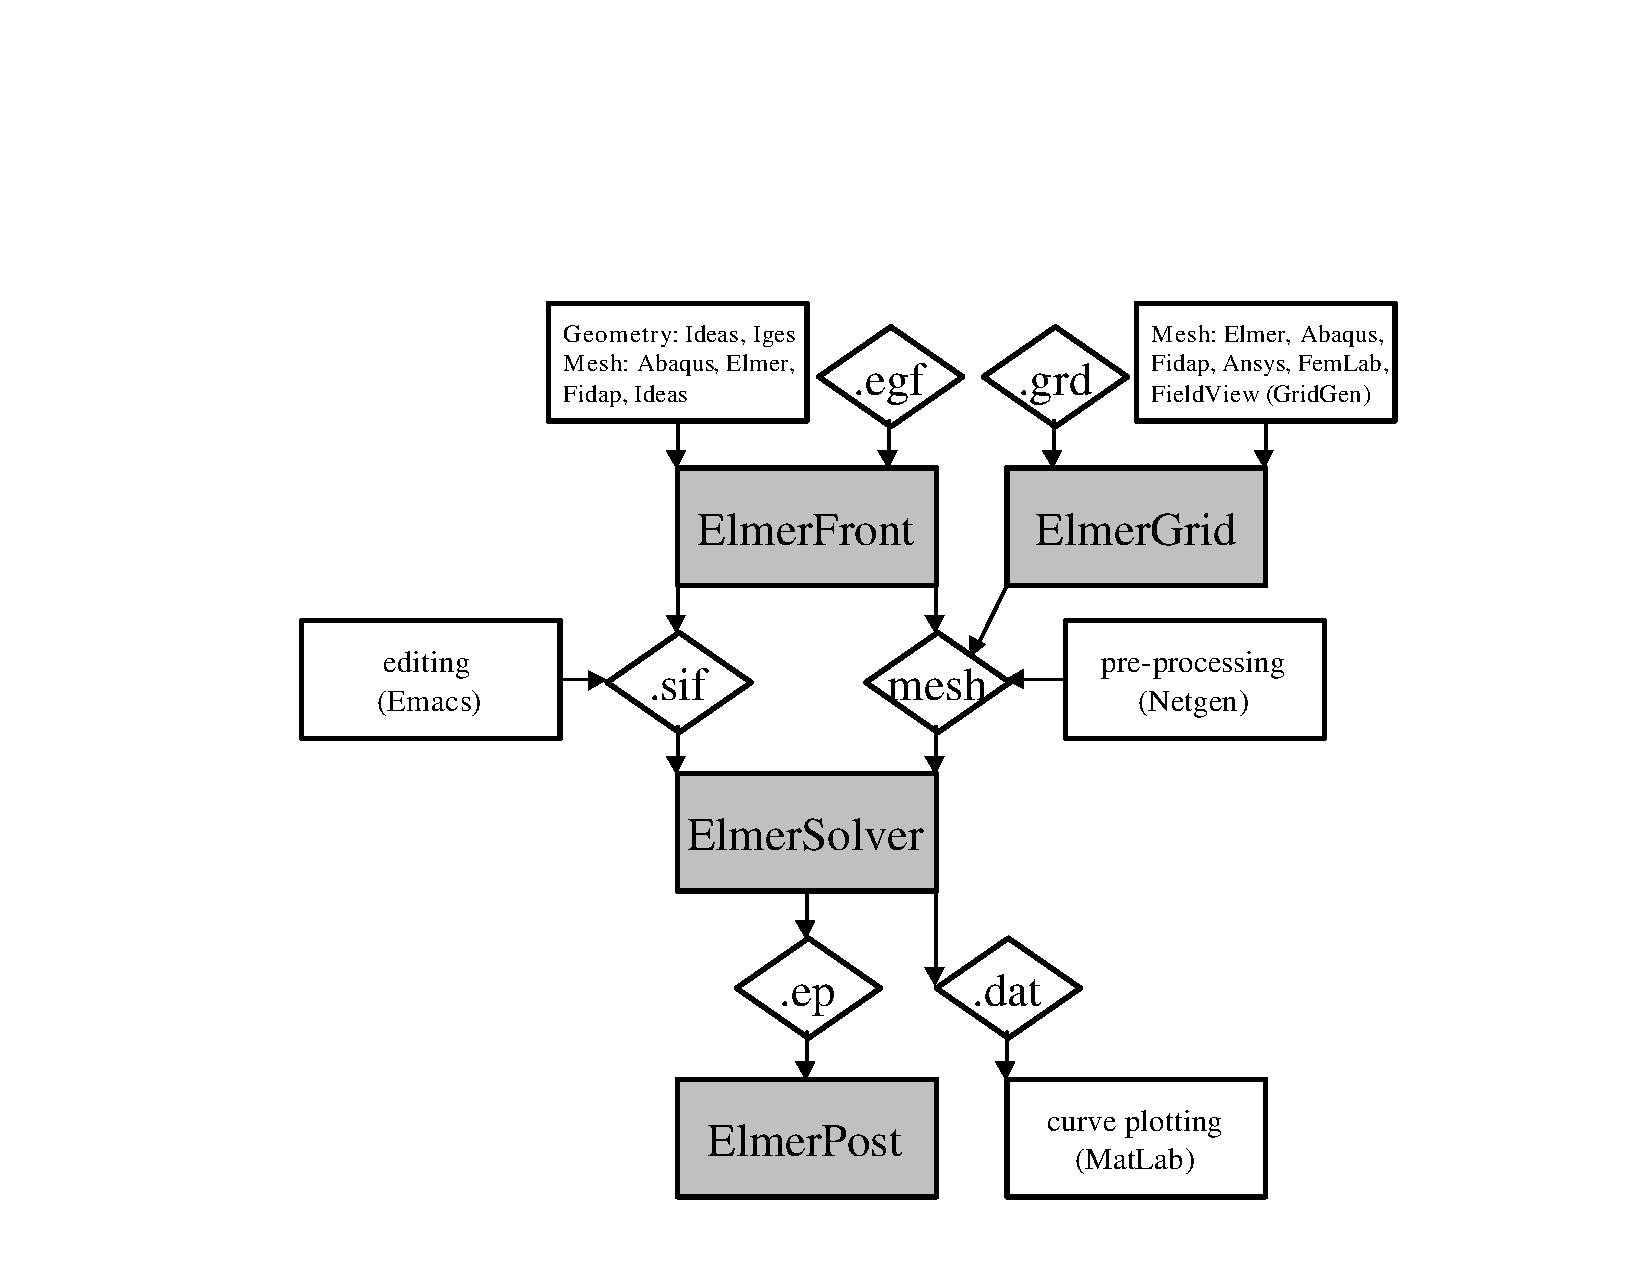
\includegraphics[width=13.0cm]{elmer-chart.pdf}
\caption{Work flow in the Elmer environment}
\label{fig_workflow}
\end{center}
\end{figure}



\section{Strategies for using the Elmer package}

The modularity of the Elmer package enables the users to have different strategies 
for using Elmer. Figure~\ref{fig_workflow} shows schematically how the key
software components depend on one another. Here the possible ways of using
the package are outlined. How the input and output data of the software components
are organized into files is also summarized.

%Because of the number of different modules in Elmer there is a number of different strategies
%how use Elmer. 
%Here we try to explain the different choices in more detail. 
%Examples on the different choices strategies may be found in Elmer tutorials. 
%Figure~\ref{fig_workflow} shows a schematic pictures on how the different components depend
%on one-another.


\subsection{Elmer file system}

The following list summarizes how the input and output data are organized into files.

%\section{Elmer file formats}
%Elmer uses and creates variable number of files in the solution of the case. 
%Here is some information about the Elmer file system. 

\sifbegin
\sifitem{ElmerSolver command file}{*.sif}
The file with the sif-suffix is the command file which is read by ElmerSolver.
It contains user-prepared input data that controls the selection of physical models,
boundary conditions, and so on. In the case of simple problem setups this command file 
may be written automatically by ElmerFront. More complicated setups require that this 
file is edited using a text editor. The documentation of the software includes several
example files that may be used as starting points when editing the command file.
For the keyword syntax of the command file
the ElmerSolver Manual and Models Manual are the best sources of information.

\sifitem{ElmerSolver mesh files}{mesh.*}
The solver of Elmer reads the mesh from four different files \texttt{mesh.nodes},
~\texttt{mesh.elements},\linebreak[4] \texttt{mesh.boundary}, and \texttt{mesh.header},
which all should be located in a single mesh directory. The mesh files may be created using 
ElmerFront, ElmerGrid, or by enhanced versions of Netgen and GiD. A program executable
Mesh2D which is the mesh generator used by ElmerFront may also be called independently.
The file format of the mesh files is compatible with ElmerSolver, ElmerFront and ElmerGrid.

\sifitem{ElmerSolver result file}{*.result}
This result file is written by ElmerSolver and may be used to make a simulation 
restart from a previous set of results. ElmerSolver by default writes this file to 
the mesh directory. The file format is compatible only with ElmerSolver.

\sifitem{ElmerPost file}{*.ep}
This file is written by ElmerSolver and can be read by ElmerPost. 
ElmerSolver by default writes this file to the mesh directory.
The file is used mainly for visualization purposes.

\sifitem{Elmer geometry file}{*.egf}
This file defines a 2D geometry using primitives such as points and lines.
It is read by the ElmerFront program and can be edited using a text editor.

\sifitem{Elmer mesh generator input file}{*.mif}
This is the file that Mesh2D uses to create Delaunay triangulations. 
It is usually written by ElmerFront but it may easily be modified using an editor.

\sifitem{ElmerGrid mesh definition file}{*.grd}
This file is used to define 1D, 2D or 3D structured meshes. 
The file can only be read by ElmerGrid.

\sifitem{ElmerGrid command file}{*.eg}
This file is used to make mesh manipulation operations with ElmerGrid. The same functionality 
may be achieved by using command line arguments.

\sifitem{ELMERSOLVER\_STARTINFO}{} 
This file is used by ElmerSolver and simply includes the name of the command file.
The other possibility to transfer the command file name to ElmerSolver is to use 
a command line parameter.

\sifitem{SOLVER.KEYWORDS}{}
The keywords that may be used in the ElmerSolver command file are listed in this file, located 
in the directory of the shared library files of ElmerSolver. This list may not be complete as new keywords 
are always popping up due to the development work. Therefore the user may create a local file and 
add the missing keywords to this file. Note that it does not really matter if a keyword is not listed
as long as the type of the keyword value is given in the command file and ElmerSolver is not asked to
do a strict checking of keywords. 
%; see the documentation of the \texttt{check keywords warn} keyword.
%in the command file the \texttt{Check Keywords Warn} is used 
%instead of \texttt{abort}. 

\sifend 


\subsection{Strategies for preprocessing}

The purpose of the preprocessing phase is to create the ElmerSolver input files, which 
are at the minimum the command file and the mesh files. 


\subsubsection*{Geometry definition + ElmerFront}

The simplest way to create a simulation from scratch is to use an existing 
geometry definition (egf or 2D CAD file) and ElmerFront. After reading the geometry data,
ElmerFront may be used to create the mesh and define the equations, boundary and initial conditions, 
and material parameters. The functionality of ElmerFront is not actually limited to 
preprocessing tasks, since the program executables for the solution and the visualization of the results 
(ElmerSolver and ElmerPost) can also be started via ElmerFront.
%For the solution ElmerFront calls ElmerSolver automatically, and likewise ElmerPost for the visualization. 

A handicap with ElmerFront is that it does not have any geometry definition tools,
and the mesh generation tools are limited to 2D Delaunay. In addition,
a large portion of the capabilities of ElmerSolver are not supported by ElmerFront. 
Therefore using ElmerFront as the only strategy is best suited for relatively simple tasks 
with some standard equations (heat, flow, stress). The benefit of this approach 
is that the user does not need to get acquainted with the different file formats, 
nor edit the files by hand. However, serious users have to abandon this approach as the only strategy quite soon. 


\subsubsection*{Your favorite mesh generator + ElmerFront}

Besides of its own meshing capabilities ElmerFront can read  
an existing 2D or 3D mesh. The supported formats include Abaqus, 
Fidap neutral file, Ideas universal file and Elmer mesh files. 


\subsubsection*{Editing command files created by ElmerFront}

ElmerFront may be used as a first-step tool in the simulations, even though in most of the cases it 
cannot be used for creating the full setup of the case. Making a preliminary command file and/or mesh with 
ElmerFront often saves some time. Thereafter this command file (*.sif) may be modified by some
text editor (e.g. emacs) to account for more detailed specification. In adding the keywords in the
command file, the Models Manual is of great help. In this approach ElmerSolver and ElmerPost 
are to be executed from the command line. 


\subsubsection*{ElmerGrid + editor}

An easy way to make simple 2D and 3D meshes is to use ElmerGrid. The mesh definition file 
of ElmerGrid also defines the geometry. However, the structured format of ElmerGrid favors
box-like forms and making more complicated shapes may be difficult. In this approach 
the solver command file must be created using a text editor. Previous command files provide a good 
starting point also in this case.

This approach is most suited for making academic tests using simple structured meshes. 
It is easy to test different things in this approach as the mesh is basically fully parameterized. 
Trying to push this approach to more complicated shapes may turn out to be cumbersome. 
 

\subsubsection*{Your favorite mesh generator + ElmerGrid + editor}

For more complicated geometries you may use your favorite meshes and import them into 
Elmer format using ElmerGrid. ElmerGrid can handle a number of formats different from those supported 
by ElmerFront (e.g. Ansys, Comsol, Gmsh). This procedure for importing meshes is currently
in focus in Elmer development. 
The parsers are often written case-by-case and typically no documentation is published. 
Therefore if problems arise contact the elmer team.

Even though the import of complicated meshes is quite straightforward, it may be more difficult to 
write a ElmerSolver command file for the mesh. This is particularly true if the mesh includes several bodies and 
tens of different boundary conditions. This problem could be helped by conserving name information 
throughout the import process. This is currently supported for FDNEUT and Ansys script formats.  
However, in the case of complicated geometries writing the setup with a text editor
will still be laborious.


\subsubsection*{GiD/Netgen + editor}

There is a small number of third party mesh generators that can directly write meshes in Elmer format
provided that some interfaces are used. Currently interfaces for GiD and Netgen are provided. 
For more information on the interfaces see the Elmer www-pages. 
Also here only the mesh is transformed and the solver command file must be written separately.



\subsection{Strategies for postprocessing}

There are also several strategies for visualizing the numerical results.

\subsubsection*{ElmerPost}
The easiest way for visualization is to use ElmerPost. ElmerPost does not pose any severe limitations.
However, if you want to draw line graphs, or want to have several data sets available at the same
time, you need other file formats as well. Also the vector format output (postcript)
for complicated geometries leaves something to be desired. 

\subsubsection*{VTK, GiD etc.}
ElmerSolver can write the results also in formats understood by some third party visualization 
software. Use the \texttt{ResultOutputSolve} keyword (see Elmer Models Manual) for outputting 
in VTK legacy (Visit, Paraview,\ldots ) or GiD format.

\subsubsection*{Matlab, gnuplot, etc.}
Ascii data for producing line graphs can be written automatically by saving the 
solution data along predefined lines, or lines that are created on-the-fly.
For this purpose use the \texttt{SaveLine} keyword (see Elmer Models Manual).


\section*{Contact info}

For questions concerning the use and capabilities of Elmer, 
please use preferably the Elmer discussion mailing list at \texttt{elmerdiscussion@postit.csc.fi}.

%\mbox{}\newline\noindent
%You can contact also directly some of the Elmer developers:
%\begin{itemize}
%\item Lyly Mikko, mikko.lyly@csc.fi
%\item Mika Malinen, mika.malinen@csc.fi
%\item Pursula Antti, antti.pursula@csc.fi
%\item Ruokolainen Juha, juha.ruokolainen@csc.fi
%\item R�back Peter, peter.raback@csc.fi
%\end{itemize}